% Header Part %
%^V^V^V^V^V^V^V
\documentclass[12pt,a4paper]{article}
\usepackage[margin=1in]{geometry}
%\usepackage[left=1.5in,right=1in,top=1in,bottom=1in]{geometry}
%\usepackage[utf8]{inputenc}
\usepackage{graphics,graphicx}
\usepackage{url}
\linespread{1.5}

% Body Starts from here %
%^V^V^V^V^V^V^V^V^V^V^V^V
\begin{document}
% Cover Page %
%^V^V^V^V^V^v^
\thispagestyle{empty} % No page number on the cover page
\begin{center}
\Large {\it A Report on}\\
\vspace{1cm}
\Huge {\bf Cryptoware: Rabin PKC(256 bits)}\\
\Large {(Mini-Project of CSE1007-Introduction to Cryptography)}\\
\vspace{1in}
\Large {\it Submitted by}\\
\Large {\bf Datta Sai Jadeep Varanasi}\\
\large {\bf (Registration-19BCN7035)}\\
\Large {\it on}\\
\Large {\bf 15 11 2020}\\
\vspace{2in}
\includegraphics[width=3in]{logo.jpg}\\
\vspace{1in}
\Large {\bf School of Computer Science and Engineering}\\
\Large {\bf VIT-AP University, Andhra Pradesh}\\
\end{center}

\newpage % New Page

\begin{abstract}
Every person like to share information securely so that they can
share privately. 
Cryptography is the practise and study of techniques
for secure communication in the presence of third parties. The
necessity and the fact that exchanged messages are exposed to
other people during the transmission promoted the creation of
encryption systems, enabling just the recipients to interpret the
exchanged information.
In this report, a particular cryptosystem called Rabin
Cryptosystem is presented in a client-server model and analysed with
the help of Chinese Reminder Theorem.
It first presents the algorithm for Rabin Public key encryption
then it's code in programming language and finally, the outputs of
sender's and receivers are given.
\end{abstract}

\section{Introduction}
Rabin cryptosystem is an asymmetric cryptographic
technique, whose security, like that of RSA, is related to the
difficulty of factorization. However the Rabin cryptosystem has
the advantage that the problem on which it relies has been proved
to be as hard as integer factorization.

 Asymmetric key cryptography uses two set of keys,public key and a
 private key.The public key shall be announced to everyone and
 private key is know only between the sender and receiver. The
 public key encrypts the given plain text and the private key
 decrypt's the cipher text received. If someone was able to decrypt
 the cipher text by brute force method. He ends up with multiple
 ,meaning full plain text.Only the receiver can chose the right
 plain text.

\subsection{About}
The Rabin cryptosystem is a variant of RSA cryptosystem.In RSA
cryptosystem, function used for encryption is:F(m,k)=mk(modn), where
n is a product of two large prime numbers(p,q). If k=2, then, it
becomes the encryption function of Rabin cryptosystem.
So, the decryption function becomes,sqrt(c)(mod n).During the
decryption we need to use the Extended Euclidean algorithm.

Extended Euclidean algorithm:
The extended Euclidean algorithm is an algorithm to compute integers x and y such that
ax + by = gcd(a,b)
given a and b.

n is the public key and (p,q) is the private key.
This project focuses on the Generation of public and private keys,
Implementation of encryption algorithm and also decryption algorithm.
 
\subsection{Implementation Environment}
I use JDK 9.0.4 for compiling the Rabin code.The code is in java
language.The inputs consist of two very large prime numbers,because the
larger the value the longer it takes to decrypt using brute-force
method.These two primes,p and q, give N when both are multiplied.
In this project, the key size used is 256 bit.

The extended Euclidean algorithm is used to between public key and plain text to check whether their GCD=1.
At the end of decryption, we get 4 integers d1,d2,d3,d4.
\section{Procedure}
Algorithm 1: Rabin-p Key Generation Algorithm

1:Generate two very large prime numbers, p and q, which satisfies the
  condition
  
  For example:
  p=139 and q=191
  
  Actually both the prime are taken in random and they are very large
  
  2:Calculate the value of n
   n = p.q
   
3:Publish n as public key and save p and q as private key

Algorithm 2 Rabin-p Encryption Algorithm

1:Get the public key n.

2:Convert the message to ASCII value. Then convert it to binary and
  extend the binary value with itself, and change the binary value back
  to decimal m.
  
3:Encrypt with the formula:C = m2 mod n

4:Send C to recipient.

Algorithm 3 Rabin-p Decryption Algorithm

1:Accept C from sender.

2:Specify a and b with Extended Euclidean GCD such that, a.p + b.q = 1

3:Compute r and s using following formula:
  r = C(p+1)/4 mod p
  s = C(q+1)/4 mod q
  Now, calculate X and Y using following formula:
  X = ( a.p.r + b.q.s ) mod p
  Y = ( a.p.r – b.q.s ) mod q
  The four roots are, m1=X, m2=-X, m3=Y, m4=-Y
  
4:Now, Convert them to binary and divide them all in half.

5:Determine in which the left and right half are same. Keep that
  binary’s one half and convert it to decimal m. Get the ASCII
  character for the decimal value m. The resultant character gives the
  correct message sent by sender.
  
  These Algorithms are shown at the end of the report.
\section{Major Components}
This project just shows the major components of the code.The key size is 256 bits
\begin{verbatim}
    public static void main(String[] args) 
    { 
        BigInteger[] key = Cryptography.generateKey(256);//key-size is //256bit 
        BigInteger n = key[0]; 
        BigInteger p = key[1]; 
        BigInteger q = key[2]; 
        String finalMessage = null; 
        int i = 1; 
        String s = "I am Jaideep"; 
  
        System.out.println("Message sent by sender : " + s); 
  
        BigInteger m 
            = new BigInteger( 
                s.getBytes( 
                    Charset.forName("ascii"))); 
        BigInteger c = Cryptography.encrypt(m, n); 
  
        System.out.println("Encrypted Message : " + c); 
  
        BigInteger[] m2 = Cryptography.decrypt(c, p, q); 
        for (BigInteger b : m2) { 
            String dec = new String( 
                b.toByteArray(), 
                Charset.forName("ascii")); 
            if (dec.equals(s)) { 
                finalMessage = dec; 
            } 
            i++; 
        } 
        System.out.println( 
            "Message received by Receiver : "
            + finalMessage); 
    } 
    
    public static BigInteger[] generateKey(int bitLength) 
    { 
        BigInteger p = blumPrime(bitLength / 2); 
        BigInteger q = blumPrime(bitLength / 2); 
        BigInteger N = p.multiply(q); 
        return new BigInteger[] { N, p, q }; 
    } 
  
    public static BigInteger encrypt(BigInteger m, 
                                     BigInteger N) 
    { 
        return m.modPow(TWO, N); 
    } 
  
    public static BigInteger[] decrypt(BigInteger c, 
                                       BigInteger p, 
                                       BigInteger q) 
    { 
        BigInteger N = p.multiply(q); 
        BigInteger p1 = c.modPow(p 
                                     .add(BigInteger.ONE) 
                                     .divide(FOUR), 
                                 p); 
        BigInteger p2 = p.subtract(p1); 
        BigInteger q1 = c.modPow(q 
                                     .add(BigInteger.ONE) 
                                     .divide(FOUR), 
                                 q); 
        BigInteger q2 = q.subtract(q1); 
  
        BigInteger[] ext = Gcd(p, q); 
        BigInteger y_p = ext[1]; 
        BigInteger y_q = ext[2]; 
  
        BigInteger d1 = y_p.multiply(p) 
                            .multiply(q1) 
                            .add(y_q.multiply(q) 
                                     .multiply(p1)) 
                            .mod(N); 
        BigInteger d2 = y_p.multiply(p) 
                            .multiply(q2) 
                            .add(y_q.multiply(q) 
                                     .multiply(p1)) 
                            .mod(N); 
        BigInteger d3 = y_p.multiply(p) 
                            .multiply(q1) 
                            .add(y_q.multiply(q) 
                                     .multiply(p2)) 
                            .mod(N); 
        BigInteger d4 = y_p.multiply(p) 
                            .multiply(q2) 
                            .add(y_q.multiply(q) 
                                     .multiply(p2)) 
                            .mod(N); 
        return new BigInteger[] { d1, d2, d3, d4 }; 
    } 
\end{verbatim}

\section{Results}
The above Rabin-code with key-size 256 bits encrypts the plain-text "I
am Jaideep" the encrypted-text is
"512187119936664680072072976196217771540704614274357629184"
\ref{fig:Alice}, \ref{fig:Bob}, \ref{fig:Output}, \ref{fig:keygeneration}, \ref{fig:Encrypt}, \ref{fig:Decrypt} and \ref{fig:Alice and Bob}
\begin{figure}[htbp]
  \centering
  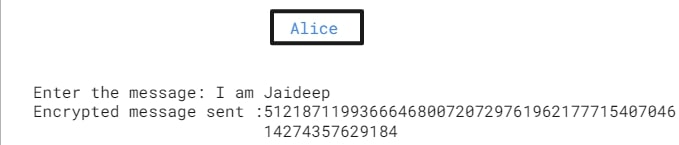
\includegraphics[width=4in]{Alice.jpg}
  \caption{Computations at Sender-side (Alice).}
  \label{fig:Alice}
\end{figure}

\begin{figure}[htbp]
  \centering
  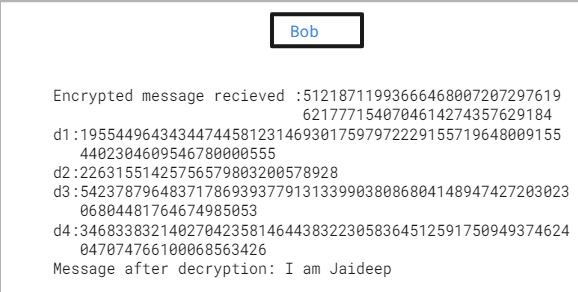
\includegraphics[width=0.5\textwidth]{Bob.jpg}
  \caption{Computations at Receiver-side (Bob).}
  \label{fig:Bob}
\end{figure}

\begin{figure}[htbp]
  \centering
  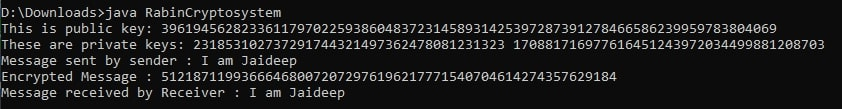
\includegraphics[width=1.1\textwidth]{Output.jpg}
  \caption{Output with public and private keys.}
  \label{fig:Output}
\end{figure}

\begin{figure}[htbp]
  \centering
  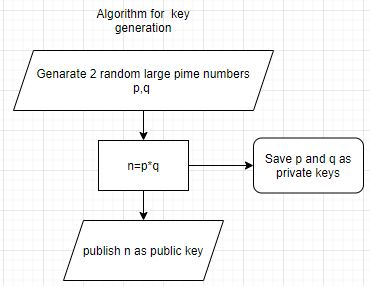
\includegraphics[width=0.5\textwidth]{keygeneration.JPG}
  \caption{Flowchart for keygeneration.}
  \label{fig:keygeneration}
\end{figure}

\begin{figure}[htbp]
  \centering
  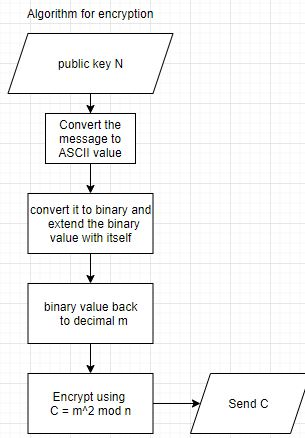
\includegraphics[width=0.5\textwidth]{Encrypt.JPG}
  \caption{Flowchart for Encryption}
  \label{fig:Encrypt}
\end{figure}

\begin{figure}[htbp]
  \centering
  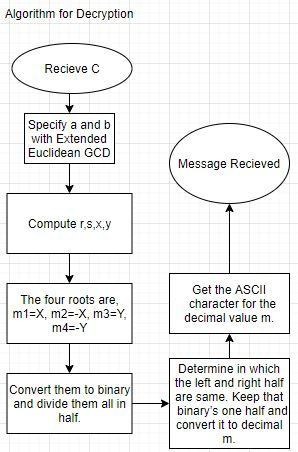
\includegraphics[width=0.5\textwidth]{Decrypt.JPG}
  \caption{Flowchart for decryption.}
  \label{fig:Decrypt}
\end{figure}

\begin{figure}[htbp]
  \centering
  \includegraphics[width=0.7\textwidth]{Alice and Bob.jpg}
  \caption{Figurative display of communication between Alice and bob.}
  \label{fig:Alice and Bob}
\end{figure}

%\begin{equation}
%   Y= f(x)
%   \label{eq:yfx}
%\end{equation}

%\begin{table}[htbp]
%    \centering
%    \begin{tabular}{|c|c|}
%    \hline
%       Name  &  RegNo\\ \hline
%       Saroj & 70051\\ \hline
%       ABCD & 1234\\ \hline
%    \end{tabular}
%    \caption{Caption}
%    \label{tab:my_label}
%\end{table}
\begin{thebibliography}{plain}

\bibitem{BForouzanBook} Behrouz A Forouzan, Debdeep Mukhopadhyay,
``Cryptography and Network Security", Mc Graw Hill, Third Edition,
2015.

\bibitem{WStallingsBook} William Stallings, ``Cryptography and Network
Security: Principles and Practice”, Pearson Education, Seventh Edition,
2017.

\bibitem{Overleaf} Overleaf: a collaborative cloud-based LaTeX editor
used for writing, editing and publishing scientific documents.
\url{http://www.overleaf.com}.

\bibitem{drawio} Drawio: a free diagramming online application used draw flowcharts,UML, entity relation, network diagrams,mockups and more. 
\url{http://draw.io/}.

\bibitem{Autodraw} Autodraw: a new web-based tool that pairs machine learning with drawings created by talented artists to help you draw
\url{https://www.autodraw.com/}.

\end{thebibliography}

\end{document}
